The properties of neutrinos summarized in the previous section pertain to those derived from the standard model. However, the latter is incomplete in its description of neutrino mass. In this section, I explain how we know neutrinos have non-zero mass and how cosmological probes can assist particle physics in determining the sum of their mass eigenstates.

\subsection{Lepton Flavour Oscillations}
\label{sec:leptonmix}


A notable counter-intuitive property\footnote{oscillations are not inherent to neutrinos; in fact, there is a misalignment between the propagating quantum states of quarks and when they partake in strong interactions.} of neutrinos is their capacity to alter their lepton charge. Predicted in 1957 by \cite{Pontecorvo57, Pontecorvo58}, the first experiment that detected these neutrino flavour oscillations can be traced back to the 1968 Homestake experiment, in which, using a chlorine-based detector, \cite{Davis68} reported a deficit in the flux of solar neutrinos with respect to the SM prediction. This deficit became known as the solar neutrino problem. Accounting for this solar deficit by flavour oscillations was made definitive in 2001 at the Sudbury Neutrino Observatory (SNO) in Ontario \citep{Sudbury_osc}. Three years prior, the Super-Kamiokande scintillator based in Japan had gathered evidence for the oscillation of flavours in atmospheric neutrinos \citep{Fukuda1998, Kajita1999}. As such, the 2015 physics Nobel prize was attributed to both Takaaki Kajita and Arthur B. McDonald for not only the detection of neutrino flavour oscillations but also evidence for non-zero neutrino masses. Indeed, if neutrinos were massless as is predicted by the SM, then, like photons, they would propagate at the speed of light and experience infinite time dilation\footnote{since their Lorentz factor $\gamma = (1-(v/c)^2)^{-1/2} \rightarrow \infty$}. Since neutrino lepton flavours oscillate, their time dilation cannot be infinite, and they therefore cannot travel at the speed of light, which means at least one neutrino eigenstate must have non-zero mass. \\

To make sense of this rather odd phenomenon, it is useful to regard the lepton charge of the neutrino as nothing more than that of the charged lepton with which it interacts via the weak force. The wave function that propagates through space in time is a time-dependent quantum superposition of \textit{mass} eigenstates $m_i = m_{1,2,3}$. When interacting, the lepton states $\nu_\ell = \nu_{e, \mu, \tau}$ are fixed superposition of those mass eigenstates:

\begin{empheq}[box=\mymath]{equation}
\displaystyle
\left\vert \nu_\ell \right\rangle = \sum\limits_{i} U^{\dagger}_{\ell i} \left\vert \nu_i \right\rangle
\end{empheq}

There is no trivial reason why these mass eigenstates should be aligned with the lepton (observed) states. In other words, the mass-flavour mixing matrix $U$, \textit{a.k.a.} the Pontecorvo–Maki–Nakagawa–Sakata (PMNS), is not diagonal. Since there are three possible lepton charges, as justified by the decay width of the $W$ boson, it is natural although arbitrary to expect three different mass eigenstates. If at least one of the eigenstates is different than the other two, then the superposition would propagate at different rates and lepton flavors are expected to oscillate.\\

\begin{figure}
\begin{center}
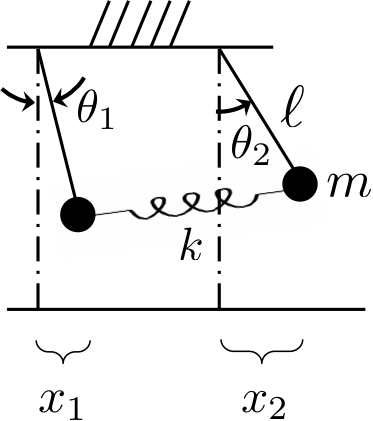
\includegraphics[width=0.25\columnwidth]{Neutrino/coupled_pendula.png}
\caption{Setup of the coupled pendula, marked by $x_1$ and $x_2$.}
\label{fig:pendulum}
\end{center}
\end{figure}

To illustrate why, it can be useful to consider the coupled pendula in Fig.~\ref{fig:pendulum}. The positions $x_1$ ad $x_2$ of the similar masses $m$ hanging in a constant gravitational field $g$ from identical lengths $\ell$ and linked by a spring of stiffness $k$ from their equilibrium positions, obey \\
\begin{equation}
\left( 
\begin{matrix}
\cfrac{d^2}{dt^2} + \cfrac{g}{\ell} + \cfrac{k}{m} & - \cfrac{k}{m} \\
- \cfrac{k}{m} & \cfrac{d^2}{dt^2} + \cfrac{g}{\ell} + \cfrac{k}{m}
\end{matrix}
\right)
\left( 
\begin{matrix}
x_1 \\
\\
x_2
\end{matrix}
\right) = \left( 
\begin{matrix}
0 \\
\\
0
\end{matrix}
\right)
\end{equation} \\ The coupled pendula system admits 2 normal modes, depicted in Fig.~\ref{fig:normal_mode}, which satisfy the eigenvalue equation, \\

\begin{equation}
x_{\pm} = x_2 \pm x_1 = a_{\pm} \cos \left( \omega_{\pm} t + \phi_{\pm} \right)
\end{equation} \\ where $\omega_{+}^2 = g / \ell$ and $\omega_{-}^2 = \omega_{+}^2 + 2 k / m$. The presence of the spring makes the natural frequency of the inverse mode, in which the masses oscillate with opposite directions, higher than that of the normal mode, in which the masses swing in unison: $\omega_{-} > \omega_{+}$. The generic solution is a superposition of both of these modes:

\begin{equation}
\label{eq:genericsol}
\left(  
\begin{matrix}
x_1 \\
x_2
\end{matrix}
\right) = \left(
\begin{matrix}
1 & 1\\
1 & -1
\end{matrix}
\right) \left(
\begin{matrix}
x_{+}\\
x_{-}
\end{matrix}
\right)
\end{equation}

\begin{figure}
\begin{center}
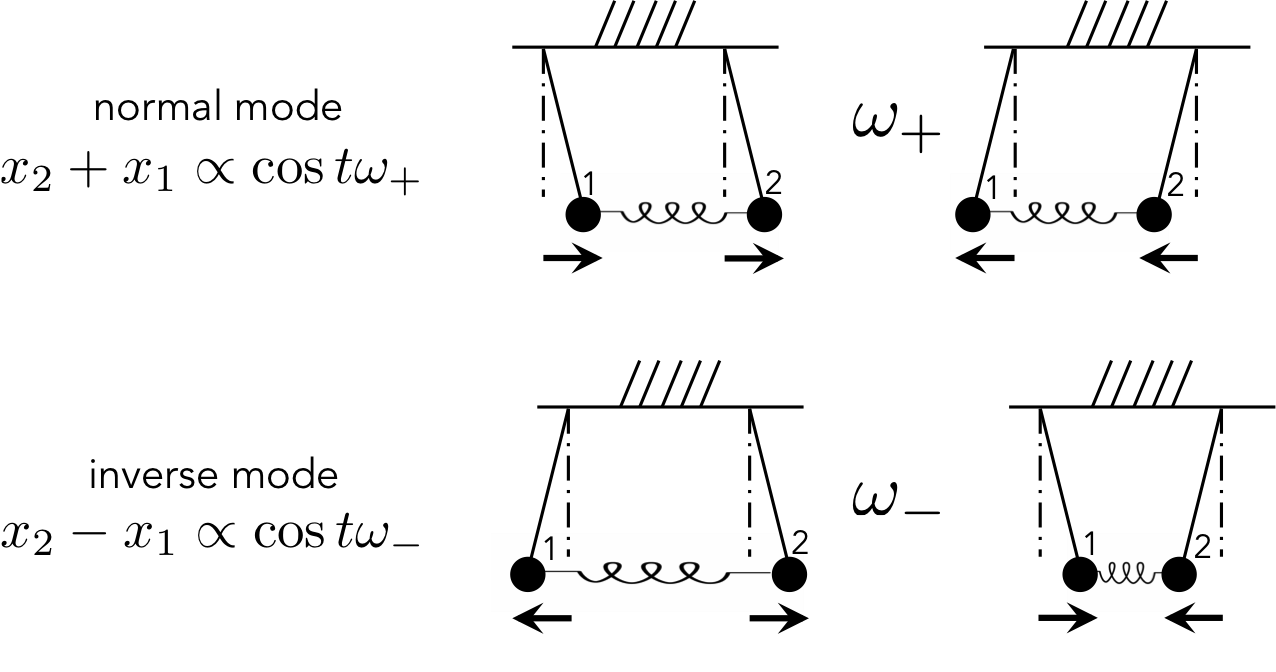
\includegraphics[width=0.85\columnwidth]{Neutrino/normal_modes.png}
\caption{The two normal modes of the coupled pendula, oscillating at frequencies $\omega_{\mp}$.}
\label{fig:normal_mode}
\end{center}
\end{figure}

Because the two modes oscillate at different frequencies, nudging the left pendulum only from its equilibrium position will inevitably result in the right pendulum swinging. The less stiff the spring or the heavier the masses, the more time the left pendulum will swing leaving the right one relatively unperturbed. After several cycles, the left pendulum's oscillations will dampen to a halt, with all the initial momentum transfered to the right one ! The oscillations of both pendula are plotted on Fig.~\ref{fig:trajectory_pendulum}. \\

\begin{figure}
\begin{center}
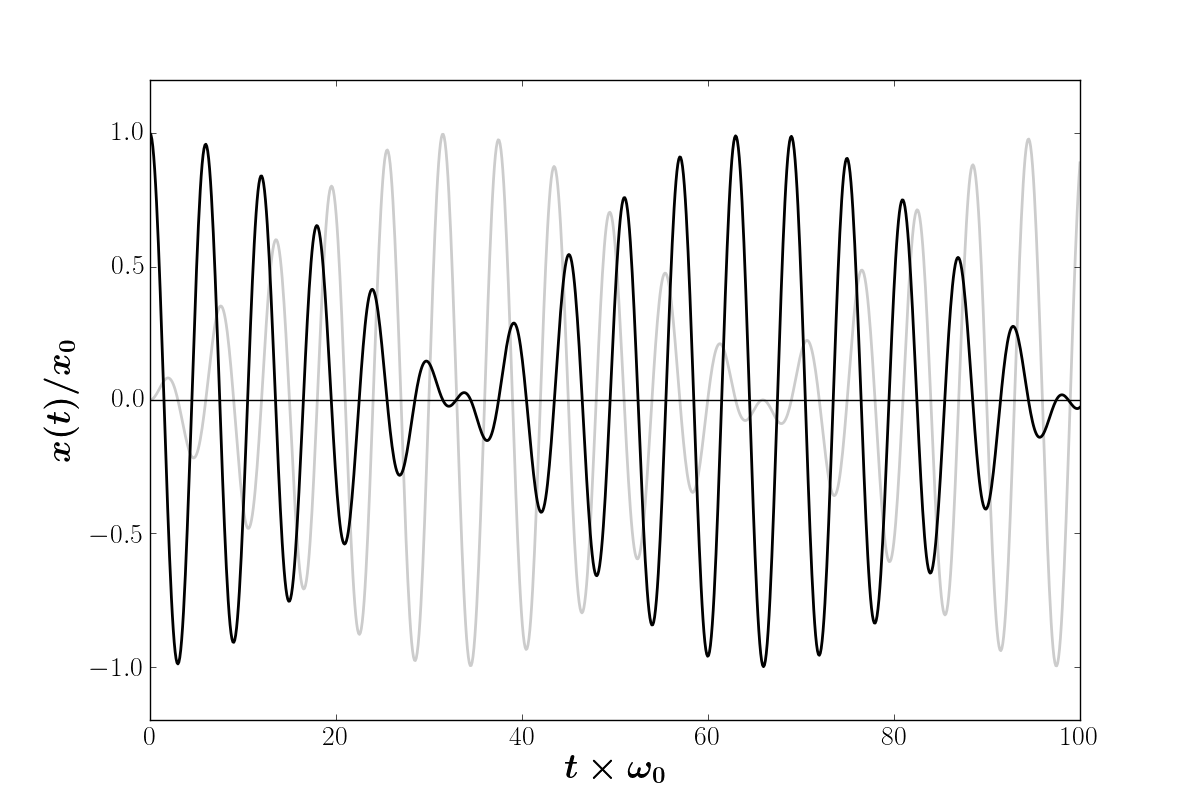
\includegraphics[width=0.85\columnwidth]{Neutrino/pendulum_x.png}
\caption{Position of the two pendula from their respective rest postitions, as a function of time. Black curve: $x_1$. Grey curve: $x_2$.}
\label{fig:trajectory_pendulum}
\end{center}
\end{figure}


\subsection{Neutrino Masses and Mixing}
\label{sec:numassmix}

\begin{figure}
\begin{center}
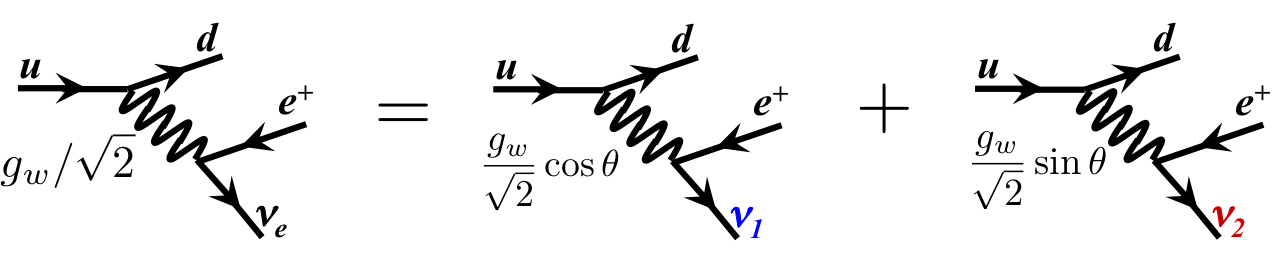
\includegraphics[width=0.9\columnwidth]{Neutrino/seesaw.png}
\caption{Feynman diagram of $\beta^{+}$ decay, producing an electron-flavoured neutrino, which can be interpreted as the superposition of two normal modes (here two mass eigenstates).}
\label{fig:mixing}
\end{center}
\end{figure}

This simple coupled pendula is analogous to neutrino flavour oscillations involving $2$ observation states $\ell = \lbrace e, \mu \rbrace$ and $2$ mass eigenstates $i = \lbrace 1, 2 \rbrace$. As Fig.~\ref{fig:mixing} illustrates, the electron neutrino produced in $\beta^{+}$ decay for instance can be described in mathematical terms as the superposition of the production of eigenstates $\nu_1$ and $\nu_2$. If one notes $\theta$ as the mixing angle between the two mass eigenstates, then 

\begin{equation}
\label{eq:2eigen}
\left( 
\begin{array}{c}
\nu_e \\
\nu_\mu \\
\end{array}
\right) = \left(
\begin{array}{cc}
c_{12} & - s_{12} \\
s_{12} & c_{12}
\end{array}
\right)
\left( 
\begin{array}{c}
\nu_1 \\
\nu_2 \\
\end{array}
\right)
\end{equation} \\ where $c_{12} \doteq \cos \theta$, $s_{12} \doteq \sin \theta$. Since $\cos^2 \theta + \sin^2 \theta = 1$, $c_{12}$ and $s_{12}$ can be interpreted as the interaction probability with each of the eigenstates. Notice the similarity of Eq.~\ref{eq:2eigen} and Eq.~\ref{eq:genericsol}. Each of these eigenstates is a normal mode of the coupled pendula, while the lepton states correspond to the $(x_1 = x_{\mathrm{max}}, x_2=0)$ and $(x_1 = 0, x_2 = x_{\mathrm{max}})$ configurations. Since $\theta \neq 0$, the eigenstates are misaligned and as time elapses, they propagate in space at different rates. At any given time, the probability of measuring flavour $\ell$ is given by the quantity

\begin{equation}
\label{eq:oscprob}
\left\vert \left\langle \nu_\ell \vert \nu (t) \right\rangle \right\vert^2 =  \sin^2 \left( 2 \theta \right) \times \sin^2 \left( \frac{L \Delta m^2}{4 E} \right)
\end{equation} \\ where $E$ is the energy of the eigenstate, $L$ is the distance travelled from the source, assuming it is produced in the other state than the one measured, and $\Delta m^2 = \vert m^2_2 - m^2_1 \vert$. The probability of detecting flavour $\ell$ as a function of $L/E$ can be visualized by squaring the curve in Fig.~\ref{fig:trajectory_pendulum}, in which one can distinguish two characteristic frequencies. The first right-hand term of Eq.~\ref{eq:oscprob}, \textit{i.e.} the intrinsic misalignment of the mass eigenstates, predominates the short-range oscillations; whereas the long-range oscillations forming the envelope are governed by the right-most term, and is determined by the distance from source to target. \\



Since there are three lepton charges, and at least as much mass eigenstates, then a more fitting classical analog would be three pendula coupled to each other with three (not two!) springs. Similar to Eq.~\ref{eq:2eigen}, the $3$ mass eigenstates are related to the lepton states via a $3 \times 3$ mass PMNS mixing matrix, \\


\begin{equation}
\left( 
\begin{array}{c}
\nu_1 \\
\nu_2 \\
\nu_3
\end{array}
\right) = 
U_1 U_2 U_3 \Delta
\left( 
\begin{array}{c}
\nu_e \\
\nu_\mu \\
\nu_\tau
\end{array}
\right)
\end{equation} \\ It can be decomposed into the $3$ rotation matrices between eigenstates $\nu_i$ and $\nu_j$, 

\begin{equation}
U_1 = 
\left( 
\begin{array}{ccc}
1 & 0 & 0 \\
0 & c_{23} & s_{23} \\
0 & -s_{23} & c_{23}
\end{array}
\right)~~~~~
U_2 = 
\left( 
\begin{array}{ccc}
c_{13} & 0 & s_{13}e^{i \delta} \\
0 & 1 & 0 \\
- s_{13}e^{i \delta} & 0 & c_{13}
\end{array}
\right)~~~~~
U_3 = 
\left( 
\begin{array}{ccc}
c_{12} & s_{12} & 0 \\
- s_{12} & c_{12} & 0 \\
0 & 0 & 1
\end{array}
\right)
\end{equation} \\ and a phase matrix

\begin{equation}
\Delta = 
\left( 
\begin{array}{ccc}
e^{i \alpha_1 / 2} & 0 & 0 \\
0 & e^{i \alpha_2 / 2} & 0 \\
0 & 0 & 1
\end{array}
\right)
\end{equation} \\ which yields a total of 9 neutrino parameters: \\

\begin{itemize}
\item[$\bullet$] the mixing angles $\theta_{12}$, $\theta_{13}$ and $\theta_{23}$;
\item[$\bullet$] the (squared) mass differences $\Delta m^2_{21}$, $\Delta m^2_{31}$ and $\Delta m^2_{32}$; and
\item[$\bullet$] three phases $\alpha_1$, $\alpha_2$ and $\delta$.\\
\end{itemize} 
For a $n \times n$ mixing matrix, involving $n$ detectable states and $n$ mass eigenstates\footnote{$n=4$ (\textit{resp.} $n=6$) for adding 1 (\textit{resp.} 3) sterile neutrinos in addition to the left-handed states; see Sec.~\ref{sec:numsms} for motivation}, there are $n^2$ real parameters, including $n(n-1)/2$ angles and $n(n+1)/2$ phases. Not all of the phases are physical, however. So far, for the SM $n=3$ case, neutrino experients typically probe composites of these parameters, which are grouped in Tab.~\ref{tab:neutrinoparamexp}. Only $\delta$, $\alpha_{1,2}$ and the sign of $\Delta m^2_{32}$ remain unknown (see Sec.~\ref{sec:massorder}). \\


\subsection{Mass Ordering}
\label{sec:massorder}

\begin{table}
	\begin{center}
		\begin{tabular}{ccl}
			\toprule
			\textbf{parameter} & \textbf{constraint} & \textbf{experiment type} \\
			\midrule
			$\sin^2 2 \theta_{12}$ & $0.846 \pm 0.021$ & Solar: KamLand. Acc: Minos, T2K\\
			$\sin^2 2 \theta_{13}$ & $0.093 \pm 0.008$ & Reactor: Daya-Bay, RENO, D-Chooz. Acc: Minos, T2K\\
			$\sin^2 2 \theta_{23}$ & $\geqslant 0.92$ & Acc: Minos, T2K. Atmospheric \\
			$\Delta m^2_{\mathrm{sol}}$ & $(7.53 \pm 0.18) \times 10^{-5}~\mathrm{eV}^2$ & Solar: KamLAND \\
			$\Delta m^2_{\mathrm{atm}}$ & $(2.44 \pm 0.06) \times 10^{-3}~\mathrm{eV}^2$ & Atmospheric \\
			\bottomrule
		\end{tabular}
	\end{center}
	\caption{Current constraints on neutrino parameters. Quoted uncertainties are $1 \sigma$ when around a best fit value, and $90\%$ likelihood when lower bound. $\Delta m^2_{\mathrm{sol}} = \Delta m^2_{21}$ and $\Delta m^2_{\mathrm{atm}} = \vert \Delta m^2_{32} \vert \simeq \vert \Delta m^2_{31} \vert$. From \cite{PDG} and \cite{W_decay_width}.}
	\label{tab:neutrinoparamexp}
\end{table}

Although neutrino flavour oscillations involve $3$ mass eigenstates and $3$ lepton measured states, the measurement probability for the $n=2$ case in Eq.~\ref{eq:oscprob} can be used as an approximation to the oscillations between $\nu_{\mu} \longleftrightarrow \nu_{\tau}$ in atmosphere neutrinos, since $\nu_e$ are seldom involved. It also approximates solar neutrino oscillations, in which $\nu_e$ oscillate into a superposition of $\nu_\mu$ and $\nu_\tau$. These approximations are valid since $\theta_{13} \ll 1$ (see Tab.~\ref{tab:neutrinoparamexp}) and because two of the eigenstates are similar in mass relative to the remaining third one. \\

By convention, the mass eigenstates are labelled such that $\vert U_{e1} \vert^2 \geqslant \vert U_{e2} \vert^2 \geqslant \vert U_{e3} \vert^2$, implying that the $\nu_1$, $\nu_2$ and $\nu_3$ have decreasing components of $\nu_e$ in that order. With such convention, the solar neutrino oscillations are governed by $\Delta m^2_{21}$, as $\nu_{1,2}$ are `` electron-rich ''; whereas the atmospheric neutrino oscillations are governed by the other two squared mass difference. \cite{Sudbury_osc} established in the SNO experiment that $\Delta m^2_{21} > 0$. However, it is still unclear today whether $m^2_3 > m^2_2$ or $m^2_3 < m^2_1$, each case being known as the normal and inverted ordering respectively, illustrated in Fig.~\ref{fig:hier}. To determine the absolute scale of neutrino masses, one can go about two ways: measure either\\

\begin{itemize}
\item[$\bullet$] the lightest mass state, which can be deduced from an effective mass $m^2_\beta = \displaystyle\sum_{i=1}^{3} U_{e i} m^2_i$ probed by the products of $\beta$ decay from tritium $^3_1 \mathrm{H}$, attempted by experiments such as KATRIN \citep{KATRIN}; or\\

\item[$\bullet$] the sum of all three eigenstates $\sum m_\nu = m_1 + m_2 + m_3$, which is attempted by cosmological probes such as the Cosmic Microwave Background or, as is the case in this work, the Lyman-alpha forest.
\end{itemize}

\begin{figure}
\begin{center}
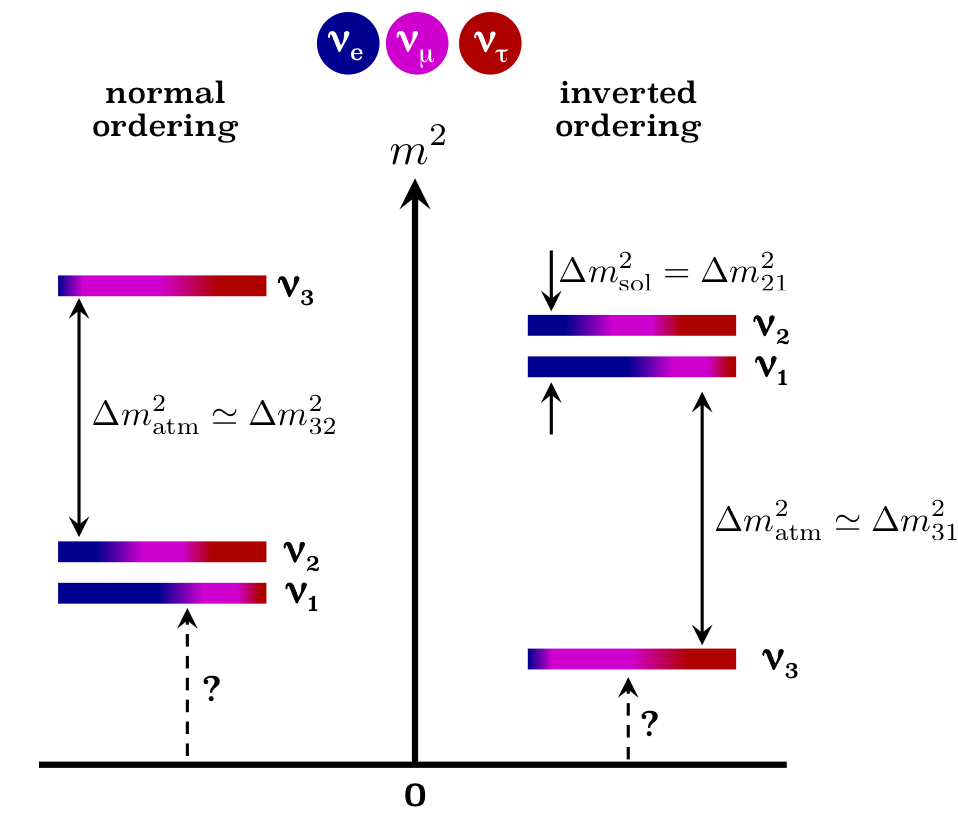
\includegraphics[width=0.6\columnwidth]{Neutrino/hierarchy.png}
\caption{Normal (left) and inverted (right) neutrino mass ordering. Blue, purple and red correspond to the $\nu_{e, \mu, \tau}$ lepton states and their proportion in the mass eigenstates reflect the PMNS matrix elements.}
\label{fig:hier}
\end{center}
\end{figure}


\clearpage